\documentclass{article}

\author{Philipe Fatio}
\title{Mechanik Formelsammlung}
\date{\today}

\usepackage[
	a4paper,
	landscape,
	left=1.25cm,
	right=1.25cm,
	top=0.75cm,
	bottom=0.75cm,
	includeheadfoot
]{geometry}

\usepackage{multicol}
\setlength{\columnseprule}{.5pt}
\setlength{\columnsep}{1cm}
\setlength{\parindent}{0cm}

%\usepackage{graphics}
\usepackage{graphicx}
\usepackage{wrapfig}
\usepackage{pdfpages}

\usepackage[all]{xy}

\usepackage{empheq}

\usepackage{fancybox}
\setlength\shadowsize{1.5pt}

% Wir schreiben hier auf Deutsch
\usepackage[german]{babel}

% Use utf-8 encoding for foreign characters
\usepackage[utf8]{inputenc}

% Differential
\newcommand{\ud}{\,\mathrm{d}}

% Nice headers
\usepackage{fancyhdr}
\fancyhf{}
\cfoot{-- \emph{\thepage} --}
\rhead{\textit{Philipe Fatio \& Tobias Oechslin} -- \today}
\lhead{\textbf{Mechanik Formelsammlung}}
\setlength{\headheight}{14pt}
\pagestyle{fancy}

% Use Mathematical Equations
\usepackage{amsmath}

\usepackage{titlesec}
\titleformat*{\section}{\large \bf}
\titleformat*{\subsection}{\normalsize \bf}
\titleformat*{\subsubsection}{\footnotesize \bf}
\titleformat*{\paragraph}{\footnotesize \bf}
\titleformat*{\subparagraph}{\footnotesize \bf}

\begin{document}
	\footnotesize
	\begin{multicols*}{4}
		[\section{Grundlagen}] % (fold)
			% Trigonometrische Funktionen (fold)
			\begin{tabular}{r|ccccc}
			 	& $\mathbf{0^{\circ}}$ & $\mathbf{30^{\circ}}$ & $\mathbf{45^{\circ}}$ & $\mathbf{60^{\circ}}$ & $\mathbf{90^{\circ}}$\\
				\hline
				$\boldsymbol{\sin}$ & $0$ & $\frac{1}{2}$ & $\frac{\sqrt{2}}{2}$ & $\frac{\sqrt{3}}{2}$ & $1$\\
				$\boldsymbol{\cos}$ & $1$ & $\frac{\sqrt{3}}{2}$ & $\frac{\sqrt{2}}{2}$ & $\frac{1}{2}$ & $0$\\
				$\boldsymbol{\tan}$ & $0$ & $\frac{\sqrt{3}}{3}$ & $1$ & $\sqrt{3}$ & Pol\\
			\end{tabular}
			% Trigonometrische Funktionen (end)
			\subsection{Zylindrische Koordinaten} % (fold)
				\begin{align*}
					\underline{r}(t) &= \rho(t) \, \underline{e}_{\rho} + z(t) \, \underline{e}_z \\
					\underline{v} &= \dot{\underline{r}} = \dot{\rho} \, \underline{e}_{\rho} + \rho \, \dot{\varphi} \underline{e}_{\varphi} + \dot{z} \, \underline{e}_z \\
					\underline{e}_{\rho} &= \cos{\varphi} \, \underline{e}_x + \sin{\varphi} \, \underline{e}_y \\
					\underline{e}_{\varphi} &= - \sin{\varphi} \, \underline{e}_x + \cos{\varphi} \, \underline{e}_y
				\end{align*}
				\[
					\begin{array}{r@{\:=\:}l|r@{\:=\:}l}
						x & \rho \cos{\varphi} & \rho & \sqrt{x^2 + y^2} \\
						y & \rho \sin{\varphi} & \varphi & \arctan{\frac{y}{x}} \\
						z & z & z & z
					\end{array}
				\]
			% Zylindrische Koordinaten (end)
			\subsection{Sphärische Koordinaten} % (fold)
				\begin{align*}
					\underline{r}(t) &= r(t) \underline{e}_r(t) \\
					\underline{v} &= \dot{\underline{r}} = \dot{r} \underline{e}_r + r \dot{\theta} \underline{e}_{\theta} + r \sin{\theta} \dot{\psi} \underline{e}_{\psi} \\
					\underline{e}_r (t) &= \sin{\theta} \cos{\psi} \underline{e}_x + \sin{\theta} \sin{\psi} \underline{e}_y + \cos{\theta}\underline{e}_z \\
					\underline{e}_{\theta} (t) &= \cos{\theta} \cos{\psi} \underline{e}_x + \cos{\theta} \sin{\psi} \underline{e}_y - \sin{\theta}\underline{e}_z \\
					\underline{e}_{\psi} (t) &= -\sin{\psi} \underline{e}_x + \cos{\psi} \underline{e}_y
				\end{align*}
				\[
					\begin{array}{r@{\:=\:}l|r@{\:=\:}l}
						x & r \cos{\varphi} \sin{\theta} & r & \sqrt{x^2 + y^2 + z^2} \\
						y & r \sin{\varphi} \sin{\theta} & \varphi & \arctan{\frac{y}{x}} \\
						z & r \cos{\theta} & \theta & \arctan{\frac{\sqrt{x^2 + y^2}}{z}}
					\end{array}
				\]
			% Sphärische Koordinaten (end)
			\subsection{Geschwindigkeit \& Schnelligkeit} % (fold)
				\begin{align*}
					\underline{v} &= \dot{\underline{r}}\\
					\underline{v} &= \dot{s}\cdot\underline{\tau}\\
					\dot{s} &= |\underline{v}| = v
				\end{align*}
			% Geschwindigkeit & Schnelligkeit (end)
			\subsection{Satz der projizierten Geschwindigkeit (SdpG)} % (fold)
				Projektion zweier Geschwindigkeiten auf Verbindungsgerade ist gleich.
				\[
					\underline{v}_A \cdot \underline{AB} = \underline{v}_B \cdot \underline{AB}
				\]
			% Satz der projizierten Geschwindigkeit (SdpG) (end)
			\subsection{Rotation} % (fold)
				Bewegung um \textbf{Rotationsachse} $\mathbf{\mu}$, welche durch zwei Punkte in Ruhe geht. Jeder Punkt ausserhalb $\mu$ beschreibt Kreisbahn um $\mu$ und hat senkrechtes $\underline{v}$ dazu:
				\begin{align*}
					\underline{v}_M &= \underline{\omega} \times \underline{r}_{\mu M} \\
					\underline{\mu} &= \underline{B} + \lambda \, \underline{\omega}
				\end{align*}
				\subsubsection{Kreiselung} % (fold)
					Entspricht Rotation, wobei nur ein Punkt in Ruhe und $\underline{\mu}$ seine Richtung ändert (Funktion von $t$).
				% Kreiselung (end)
			% Rotation (end)
			\subsection{Allgemeine Bewegung} % (fold)
				\begin{empheq}[box=\shadowbox*]{equation*}
					\underline{v}_M = \underline{v}_B + \underline{\omega} \times \underline{BM}
				\end{empheq}
				\paragraph{Kinemate:} % (fold)
					$\{\underline{v}_B,\underline{\omega}\}$
				% Kinemate (end)
				\paragraph{Invarianten:} % (fold)
					Im ganzen Körper konstant.
					\subparagraph{1. Invariante:} % (fold)
						$\underline{\omega}$
					% 1. Invariante (end)
					\subparagraph{2. Invariante:} % (fold)
						\begin{align*}
							\underline{v}_{\omega} &= \left(\underline{v}_M\right)_{\omega} = \left(\underline{v}_B\right)_{\omega} \\
							\underline{\omega} \cdot \underline{v}_B &= \underline{\omega} \cdot \underline{v}_M \\
							\underline{v}_{\omega} &= \left(\underline{e}_{\zeta} \cdot \underline{v}_B\right) \underline{e}_{\zeta} \\
							\underline{e}_{\zeta} &= \frac{\underline{\omega}}{|\underline{\omega}|}
						\end{align*}
					% 2. Invariante (end)
				% Invarianten (end)
				\subsubsection{Spezialfälle} % (fold)
					\[
						\begin{array}{r@{\,}l@{\quad\Rightarrow\ }l}
							\underline{\omega} &= \underline{0} & \text{Translation} \\
							\underline{v}_B &= \underline{0} & \text{Rotation um } \mu,\, B \in \mu \\
							\underline{v}_B &\perp \underline{\omega} & \text{Rotation um } \mu,\, B \not\in \mu
						\end{array}
					\]
				% Spezialfälle (end)
				\subsubsection{Schraubung} % (fold)
					\paragraph{Zentralachse $\mathbf{\zeta}$:} % (fold)
						Schraubung um diese Gerade. Punkte darauf haben Geschwindigkeit
						$\underline{v}_{\omega}.$
						\subparagraph{Bestimmung:} % (fold)
							$B(x_B, y_B, z_B) \in K$ mit bekannter Kinemate. Zu bestimmender
							Punkt $Z(x_Z,y_Z,z_Z) \in \zeta$ mit
							$\underline{v}_Z = \underline{v}_{\omega}$.
							\[
								\underline{v}_{\omega} = \underline{v}_B + \underline{\omega} \times \mathbf{\underline{BZ}}
							\]
						% Bestimmung (end)
					% Zentralachse (end)
				% Schraubung (end)
			% Allgemeine Bewegung (end)
			\subsection{Ebene Bewegung} % (fold)
				Bahnkurve immer in der selben Ebene.
				\paragraph{Momentanzentrum $Z$:} % (fold)
					\[
						v_N = \omega \, r \ , \quad
						\text{wobei} \quad r = |\underline{ZN}| \quad
						\text{und} \quad v_Z = 0
					\]
					$Z$ befindet sich im Schnittpunkt der Senkrechten zweier
					Geschwindigkeitsvektoren.

					\subparagraph{Spezialfälle:} % (fold)
						\begin{itemize}
							\item gleiche Geschwindigkeitsvektoren \\
							$\Rightarrow$ Translation, $Z$ in $\inf$
							\item Geschwindigkeiten
							$\underline{v}_N \parallel \underline{v}_B$ und
							$\underline{v}_N \neq \underline{v}_B$: $Z$ liegt im
							Schnittpunkt der Gerade $BN$ und der Verbindungslinie der
							Vektorspitzen.
							
						\end{itemize}
						\begin{center}
							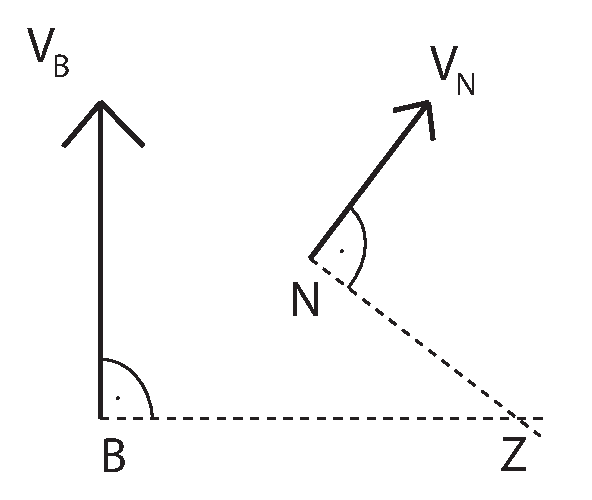
\includegraphics[width=2.5cm]{img/Zentralachse_mit_geschwindigkeit}
							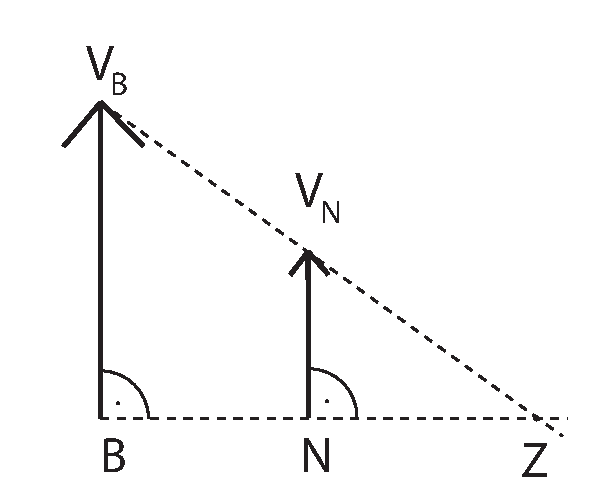
\includegraphics[width=2.5cm]{img/Zentralachse_mit_geschwindigkeit_2}
						\end{center}
					% Spezialfälle (end)
				% Momentanzentrum (end)
			% Ebene Bewegung (end)
			\subsection{Pohlbahn} % (fold)
				\paragraph{Feste Pohlbahn:} % (fold)
					Ort von $Z$ bezüglich festen Koordinatensystems ($0xy$).
					\[
						x_Z = -L \cos \varphi \ , \quad y_Z = L \sin \varphi
					\]
				% Feste Pohlbahn (end)
				\paragraph{Bewegliche Pohlbahn:} % (fold)
					\begin{gather*}
						\xi_Z = L \sin^2 \varphi = \frac{L}{2} - \frac{L}{2} \cos{2\varphi} \\
						\eta_Z = L \sin{\varphi} \cos{\varphi} = \frac{L}{2} \sin{2\varphi}
					\end{gather*}
				% Bewegliche Pohlbahn (end)
			% Pohlbahn (end)
			\subsection{Feder} % (fold)
				\[
					F(x) = k \cdot x
				\]
				$k$: Federkonstante, $x$: Ortsänderung aus der Ruhelage der Feder
				\[
					A_i = A_A
				\]
				(Arbeit innen = Arbeit aussen)
				
				Potential $V$ der inneren \emph{Federkraft} wird $U$ genannt.
				\begin{gather*}
					U = V(x) = \frac{1}{2} k x^2 \\
					V(x_0) = 0
				\end{gather*}
				$x_0$: entlasteter Zustand
				
				\subsubsection{Torsionsfeder} % (fold)
					\[
						T_R = \eta_B c_T
					\]
					$c_T$: Torsionsfederkonstante
				% Torsionsfeder (end)
			% Feder (end)
		% Grundlagen (end)
	\end{multicols*}
	\begin{multicols*}{4}
		[\section{Statik}] % (fold)
			\subsection{Kraft \& Moment} % (fold)
				\begin{align*}
					\underline{R} &= \sum_i \underline{F}_i \\
					\underline{M}_O &= \underline{OA} \times \underline{F} \\
					M_O &= |\underline{OA}| |\underline{F}| \cdot \sin{\alpha} = F \cdot a
				\end{align*}
				\[
					\underline{M}_P = \underline{M}_O + \underline{PO} \times \underline{R}
				\]
				\subsubsection{Reduktion einer Kräftegruppe} % (fold)
					\paragraph{Dyname:} % (fold)
						$\{\underline{R},\,\underline{M}_B\}$ (Kräftegruppe in beliebigem Punkt $B$ reduziert)
					% Dyname (end)
					\begin{align*}
						\textbf{1. Invariante:\ } & \underline{R} \\
						\textbf{2. Invariante:\ } & \underline{R} \cdot \underline{M}_B = \underline{R} \cdot \underline{M}_M \\
						& \underline{M}^{(R)} = \left(\underline{e}_{\zeta} \cdot \underline{M}_B\right) \underline{e}_{\zeta} \\
						& \underline{e}_{\zeta} = \frac{\underline{R}}{|\underline{R}|}
					\end{align*}
					\paragraph{Bestimmung der Zentralachse $\zeta$:} % (fold)
						\[
							\underline{M}_Z = \underline{M}_B + \underline{ZB} \times \underline{R} = \underline{M}^{(R)}
						\]
						Reduktion auf \underline{R} nur möglich, wenn
						\[
							\underline{M}^{(R)} = 0 \Rightarrow \underline{R} \cdot \underline{M} = 0.
						\]
					% Bestimmung der Zentralachse (end)
				% Reduktion einer Kräftegruppe (end)
				\subsubsection{Linienverteilte Kräfte} % (fold)
					\[
						x_S = \frac{\int_0^L x\, q(x) \ud x}{\int_0^L q(x) \ud x}
						= \frac{\int_0^L x\, q(x) \ud x}{R}
					\]
					
					\begin{wrapfigure}{r}{2cm}
						\vspace{1.25cm}
						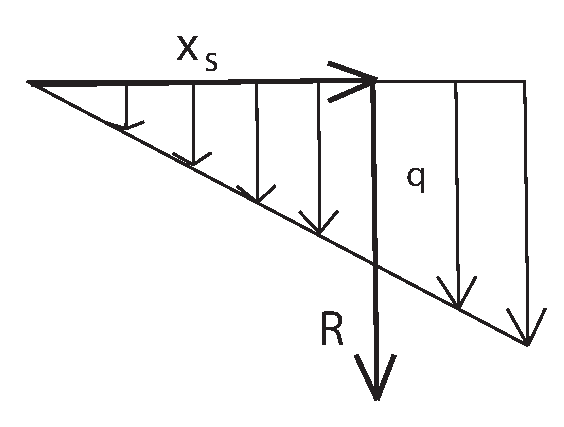
\includegraphics[width=2.5cm]{img/flaechenverteilte_kraft_im_dreieck}
						\vspace{-5cm}
					\end{wrapfigure}
					\paragraph{Sonderfälle:} % (fold)
						\begin{description}
							\item[gleichförmig:]
								$q(x) = q_0$
								
								Resultierende: $R = L \cdot q_0$
								
								Kräftemittelpunkt: $x_S = \frac{L}{2}$
							\item[dreieckförmig:]
								
								$q(x) = \frac{x}{L}q_0$
								
								Resultierende: $R = \frac{L q_0}{2}$
								
								Kräftemittelpunkt: $x_S = \frac{2L}{3}$
						\end{description}
					% Sonderfälle (end)
				% Linienverteilte Kräfte (end)
				\subsubsection{Gleichgewicht} % (fold)
					\[
						\underline{R} = \underline{0} \, , \quad \underline{M}^{(R)} = \underline{0}
					\]
				% Gleichgewicht (end)
				\subsubsection{Standfestigkeit} % (fold)

					\begin{wrapfigure}{l}{2.5cm}
						\vspace{-.75cm}
						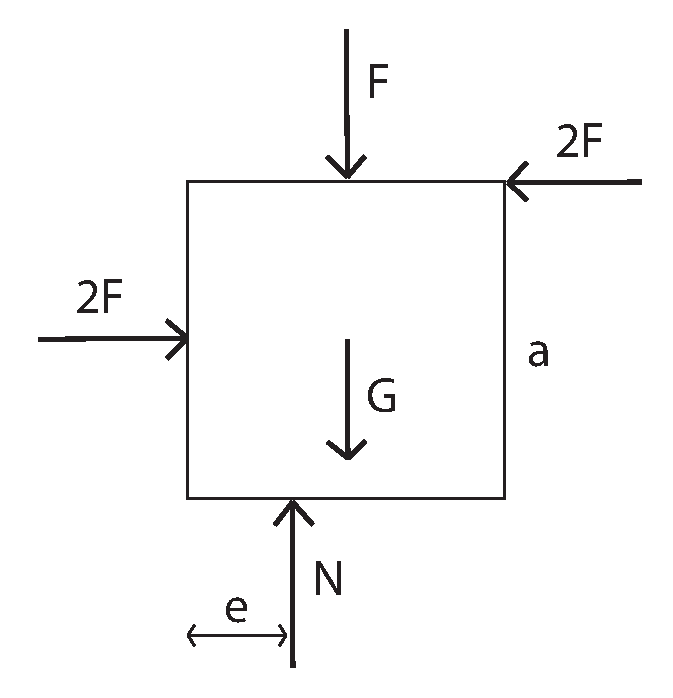
\includegraphics[width=2.5cm]{img/standfestigkeit}
						\vspace{-2.5cm}
					\end{wrapfigure}
				
					\paragraph{Bedingungen:} % (fold)
						\begin{itemize}
							\item[i)] $e > 0$
							\item[ii)] $e < a$
							\item[iii)] $N > 0$
						\end{itemize}
					
					
					% Bedingungen (end)
				% Standfestigkeit (end)
			% Kraft & Moment (end)
			\subsection{Leistung} % (fold)
				\begin{align*}
					\mathcal{P} &= \underline{F} \cdot \underline{v}_M \\
					\mathcal{P} &= |\underline{F}| |\underline{v}_M| \cdot \cos{\alpha} \\
					\mathcal{P} &= \underline{M}_O \cdot \underline{\omega}
				\end{align*}
				\subsubsection{Leistung einer Kräftegruppe} % (fold)
					\begin{align*}
						\mathcal{P}_{tot} &= \sum_i \underline{F}_i \cdot \underline{v}_i \\
						\mathcal{P}_{tot} &= \underline{v}_B \cdot \underline{R} + \underline{\omega} \cdot \underline{M}_B
					\end{align*}
				% Leistung einer Kräftegruppe (end)
				\subsubsection{Prinzip der virtuellen Leistung (PdvL)} % (fold)
					\begin{enumerate}
						\item Stab mit gesuchter Kraft entfernen und Stabkraft $s$ einführen
						\item virtueller Bewegungszustand einführen
						\item Geschwindigkeit an Knoten, wo Kräfte wirken; Winkelgeschwindigkeit für Momente
						\item Gesamtleistung $\mathcal{P}_{tot} \stackrel{!}{=} 0 \quad \Rightarrow s$ bestimmen
					\end{enumerate}
				% Prinzip der virtuellen Leistung (PdvL) (end)
			% Leistung (end)
			\subsection{Fachwerke} % (fold)
				Parallele Stäbe im Parallelogramm haben gleiches $\omega$.
				
				\emph{Lösen durch Anwendung des SdpG und PdvL.}
				
				\paragraph{Statische Bestimmtheit:} % (fold)
					\[
						2 \cdot \text{\#Knoten} = \text{\#Stäbe} + \text{\#Lagerreaktionen}
					\]
				% Statische Bestimmtheit (end)
			% Fachwerke (end)
			\subsection{Reibung} % (fold)
				%\renewcommand{\arraystretch}{1.5}
				\renewcommand{\arraystretch}{1.5}
				\addtolength{\tabcolsep}{-2pt}
				
				\hspace{-.5cm}
				\resizebox{7cm}{!} {
				\begin{tabular}{@{}rll@{}}
					 & Haftreibung & Gleitreibung \\
					\hline
					Linear     & $ |\underline{F}_R| < \mu_0 |\underline{N}| $        & $|\underline{F}_R| = - \mu_1 |\underline{N}| \frac{\underline{v}}{|\underline{v}|}$ \\
					Rollen     & $ |\underline{M}_R| < \mu_2 |\underline{N}| $        & $ |\underline{M}_R| = \mu_2 |\underline{N}| $ \\
					Gelenk     & $ |\underline{M}_R| < \mu_0 \, r_L |\underline{Z}| $ & $ |\underline{M}_R| < -\mu_1 \, r_L |\underline{Z}| \frac{\underline{\omega}}{|\underline{\omega}|} $ \\
					Längslager &  & $ |\underline{M}_{RL}| = \frac{2}{3} \mu_1 r_L |\underline{N}| $
				\end{tabular}
				}
				\renewcommand{\arraystretch}{1}
			% Reibung (end)
			\subsection{Beanspruchung} % (fold)
				\begin{align*}
					\underline{R} &= N\underline{e}_1 + Q_2 \underline{e}_2 + Q_3 \underline{e}_3 \\
					\underline{M}_C &= T \underline{e}_1 + M_2 \underline{e}_2 + M_3 \underline{e}_3
				\end{align*}
				\subsubsection{Differentialbeziehung an geraden Stabträgern} % (fold)
					\[
						\begin{array}{r@{\:=\:}l@{\, , \quad}r@{\:=\:}l}
							M_z' & -Q_y & M_y' & Q_z \\
							Q_y' & -q_y & Q_z' & -q_z \\
							M_z'' & q_y & M_y'' & q_z
						\end{array}
					\]
				% Differentialbeziehung an geraden Stabträgern (end)
				\subsubsection{Gekrümmte Beanspruchung} % (fold)
					\begin{align*}
						N &= - B_x \sin \varphi - B_y \cos \varphi \\
						Q &= B_x \cos \varphi - B_y \sin \varphi \\
						M_b &= B_x L \sin \varphi - B_y (L - L \cos \varphi)
					\end{align*}
					\begin{center}
						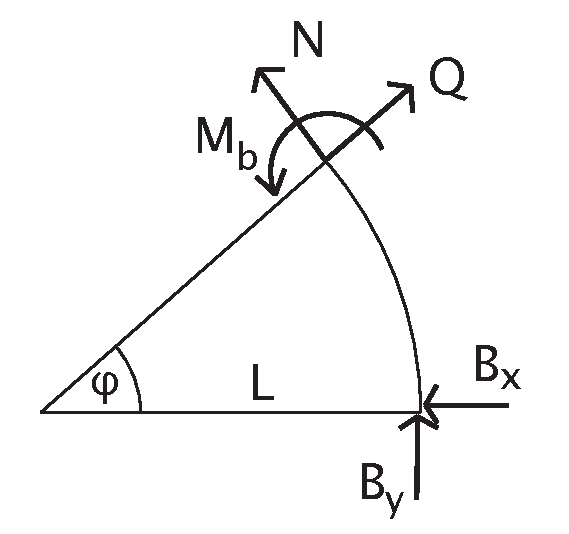
\includegraphics[width=3cm]{img/gekruemmte_beanspruchung}
					\end{center}
				% Gekrümmte Beanspruchung (end)
			% Beanspruchung (end)
		% Statik (end)
	\end{multicols*}
	\begin{multicols*}{4}
		[\section{Deformierbare Körper}] % (fold)
			\subsection{Spannung} % (fold)
				\[
					\sigma = \frac{F}{A}
				\]
				
				\begin{align*}
					[T] =& \left[\begin{array}{lll}
						\sigma_x & \tau_{xy} & \tau_{xz} \\
						\tau_{xy} & \sigma_y & \tau_{yz} \\
						\tau_{xz} & \tau_{yz} & \sigma_z
					\end{array}\right] \\
					& \mbox{\tiny $\begin{array}{ccc}
						\underbrace{ } & \underbrace{ } & \underbrace{ }  \\
						\underline{s}(\underline{e}_x) & \underline{s}(\underline{e}_y) & \underline{s}(\underline{e}_z)
					\end{array}$}
				\end{align*}
				
				$\underline{\underline{T}}$ hat Nullspalte \\
				$\quad \Rightarrow$ \textbf{Ebener Spannungszustand}
				
				Spalte ohne Schubspannung \\
				$\quad \Rightarrow$ \textbf{Hauptspannung}
				
				\[
					\underline{s} = \underline{\underline{T}} \cdot \underline{n} \quad \text{(} \underline{n} \text{ normiert)}
				\]
				
				\[
					\begin{array}{r@{\:=\:}l}
						\sigma & \underline{s} \cdot \underline{n} \\
						\underline{\sigma} & \sigma \underline{n} \\
						\tau & |\underline{s} - \sigma \underline{n}| \\
						\underline{\tau} & \underline{s} - \underline{\sigma}
					\end{array}
				\]
				\subsubsection{Gleichgewichtsbedingungen des Kontinuums} % (fold)
					\[
						\begin{array}{r@{\:+\:}r@{\:+\:}r@{\:+\:}r@{\:=\:}l}
							\sigma_{x,x} & \tau_{xy,y}  & \tau_{xz,z}  & f_x & 0 \\
							\tau_{yx,x}  & \sigma_{y,y} & \tau_{yz,z}  & f_y & 0 \\
							\tau_{zx,x}  & \tau_{zy,y}  & \sigma_{z,z} & f_z & 0
						\end{array}
					\]
				% Gleichgewichtsbedingungen des Kontinuums (end)
				\subsubsection{Mohr'scher Kreis} % (fold)
					\paragraph{Vorgehen (z.B. mit Hauptspannung in $z$):} % (fold)
						\begin{itemize}
							\item[] $\mathbf{z}\overset{\mathbf{+}}{x} \overset{\mathbf{-}}{y}$
							\item[] $
								X=\mbox{\tiny $\left(\begin{array}{r}
									\sigma_x \\
									\mathbf{+} \tau_{yx}
								\end{array}\right)$}
								,\
								Y=\mbox{\tiny $\left(\begin{array}{r}
									\sigma_y \\
									\mathbf{-} \tau_{xy}
								\end{array}\right)$}
							$
							\item[] $\sigma_M = \frac{\sigma_x + \sigma_y}{2}$
							\item[] $R = \sqrt{(\sigma_x - \sigma_M)^2 + \tau_{xy}^2}$
						\end{itemize}
						\subparagraph{Spezialfälle} % (fold)
							$\sigma_x = \sigma_y$: Kreis wird zu Punkt; alle
							Achsen = Hauptachsen; alle senkrechten Flächenelemente
							schubspannungsfrei.
							
							$\sigma_x \neq 0$, $\sigma_y = \sigma_z = 0$: einachsiger Spannungszustand (nur Druck oder Zug)
						% Spezialfälle (end)
					% Vorgehen Hauptachsen z (end)
					\paragraph{Vorgehen ohne Hauptspannungen:} % (fold)
						$\Rightarrow$ \emph{Eigenwertproblem}
						
						$k = 1,\ 2, \text{ oder } 3$ \text{(Hauptspannungen)}
						\begin{align*}
							\det([T]- \sigma_k \, I_n) &= 0 \quad \Rightarrow \text{Hauptspannungen} \\
							([T]- \sigma_k \, I_n) \underline{x} &= 0 \quad \Rightarrow \text{Eigenvektoren}
						\end{align*}
						\[
							(\sigma_k)^3 - \sigma_I (\sigma_k)^2 - \sigma_{II} \sigma_k - \sigma_{III} = 0
						\]
					% Vorgehen ohne Hauptspannungen (end)
					\paragraph{Grundinvarianten:} % (fold) 
						\begin{align*}
							\sigma_I &= \sigma_x + \sigma_y + \sigma_z \\
							&= \sigma_1 + \sigma_2 + \sigma_3 = \text{Spur}[T] \\
							\sigma_{II} &= -\sigma_x \sigma_y - \sigma_y \sigma_z - \sigma_z \sigma_x + \tau_{xy}^2 + \tau_{yz}^2 + \tau_{xz}^2 \\
							&= - \sigma_1 \sigma_2 - \sigma_2 \sigma_3 - \sigma_3 \sigma_1 \\
							\sigma_{III} &= \det[T] = \sigma_1 \sigma_2 \sigma_3
						\end{align*}
					% Grundinvarianten (end)
				% Mohrsche Kreis (end)
			% Spannung (end)
			\subsection{Verzerrung} % (fold)
				\[
					\varepsilon = \frac{F}{EA} = \frac{\sigma}{E}
				\]
				
				\[
					[E] = \left[\begin{array}{lll}
						\varepsilon_x & \varepsilon_{xy} & \varepsilon_{xz} \\
						\varepsilon_{xy} & \varepsilon_y & \varepsilon_{yz} \\
						\varepsilon_{xz} & \varepsilon_{yz} & \varepsilon_z
					\end{array}\right]
				\]
				
				\[
					\begin{array}{r@{\:=\:}l@{\, , \quad}r@{\:=\:}l@{\:=\:}l}
						\varepsilon_x & u_{x,x} & \varepsilon_{xy} & \frac{1}{2} (u_{x,y} + u_{y,x}) & \frac{1}{2} (\gamma_x + \gamma_y) \\ [1pt]
						\varepsilon_y & u_{y,y} & \varepsilon_{xz} & \frac{1}{2} (u_{x,z} + u_{z,x}) & \frac{1}{2} (\gamma_x + \gamma_z) \\ [1pt]
						\varepsilon_z & u_{z,z} & \varepsilon_{yz} & \frac{1}{2} (u_{y,z} + u_{z,y}) & \frac{1}{2} (\gamma_y + \gamma_z)
					\end{array}
				\]
				
				\subsubsection{Winkel} % (fold)
					\[
						\gamma_y = u_{x,y} \, ,\quad 
						\gamma_x = u_{y,x} \quad \text{(Winkel)}
					\]
					
					\begin{align*}
						\gamma_x &= \frac{1}{2} (\gamma_x + \gamma_y)
									+ \frac{1}{2} (\gamma_x - \gamma_y) \\
						\gamma_y &= \underbrace{\frac{1}{2} (\gamma_x + \gamma_y)}_{\mbox{\tiny $\text{Schubverzerrung}$}}
									- \underbrace{\frac{1}{2} (\gamma_x - \gamma_y)}_{\mbox{\tiny $\text{Starrkörperdrehung}$}}
					\end{align*}
				
					\[
						\varepsilon_{xy} \left\{ \begin{array}{rl}
							> 0: & \text{Winkelverkleinerung} \\
							< 0: & \text{Winkelvergrösserung}
						\end{array} \right.
					\]

					\paragraph{Totale Winkelverkleinerung (Schubwinkel):} % (fold)
						\[
							\gamma_{xy} = 2 \cdot \varepsilon_{xy}
						\]
					% Totale Winkelverkleinerung (end)
				% Winkel (end)
				
				\hspace{-.5cm}
				\resizebox{7cm}{!}{
					\begin{tabular}{@{}rcc@{}}
						 & Starrkör- & \\
						 & perbewegung & Deformation \\
						\hline \\ [-5pt]
						Translation & $\underline{u} = \left(\begin{array}{l} u_x \\ u_y \end{array}\right) $ & $ \varepsilon_x = \varepsilon_y = \varepsilon_xy = 0$ \\ [10pt]
						\hline \\ [-5pt]
						Rotation & $ \begin{array}{r@{\:=\:}l} R_{yx} & \frac{1}{2} (\gamma_x - \gamma_y) \\ [2pt] & \frac{1}{2} (u_{y,x} - u_{x,y}) \end{array}$ & $ \varepsilon_x = \varepsilon_y = \varepsilon_xy = 0 $ \\ [10pt]
						\hline \\ [-5pt]
						Dehnung & keine & $ \begin{array}{r@{\:=\:}l} \varepsilon_x & u_{x,x} \\ \varepsilon_y & u_{y,y} \\ \varepsilon_xy & 0 \end{array} $ \\ [10pt]
						\hline \\ [-5pt]
						Schubverzerrung & keine & $ \begin{array}{r@{\:=\:}l} \varepsilon_x & 0 \\ \varepsilon_y & 0 \\ \varepsilon_xy & \frac{1}{2} (u_{y,x} + u_{x,y}) \end{array}$
					\end{tabular}
				}
				
				\subsubsection{Drehung des Koordinatensystems} % (fold)
					\[
						\{n\} = \left\{\begin{array}{r}
							\cos \alpha \\
							\sin \alpha 
						\end{array}\right\}
						\ ,\quad
						\{t\} = \left\{\begin{array}{r}
							-\sin \alpha \\
							\cos \alpha 
						\end{array}\right\}
					\]
					
					\[
						[T]_{nt} = [Q]^T [T] [Q]
					\]
					
					\[
						[Q] = \left[\begin{array}{rr}
							\cos 2 \alpha & - \sin 2 \alpha \\
							\sin 2 \alpha & \cos 2 \alpha
						\end{array}\right]
					\]
					
					\begin{align*}
						\varepsilon_n &= \{n\}^T [E] \{n\} \\
						\varepsilon_{nt} &= \{t\}^T [E] \{n\}
					\end{align*}
				% Drehung des Koordinatensystems (end)
			% Verzerrung (end)
			\subsection{Linear elastisches Stoffverhalten} % (fold)
				\begin{empheq}[box=\shadowbox]{gather*}
					\begin{array}{r@{\:=\:}l}
						\varepsilon_x & \frac{1}{E} \left[\sigma_x - \nu (\sigma_y + \sigma_z)\right] + \alpha \, \Delta T \\
						\varepsilon_y & \frac{1}{E} \left[\sigma_y - \nu (\sigma_z + \sigma_x)\right] + \alpha \, \Delta T \\
						\varepsilon_z & \frac{1}{E} \left[\sigma_z - \nu (\sigma_x + \sigma_y)\right] + \alpha \, \Delta T \\
					\end{array} \\
					\begin{array}{r@{\:=\:}l}
						\varepsilon_{yz} & \frac{1}{2G} \tau_{yz} \\ [4pt]
						\varepsilon_{zx} & \frac{1}{2G} \tau_{zx} \\ [4pt]
						\varepsilon_{xy} & \frac{1}{2G} \tau_{xy}
					\end{array} \\
					\\
					\begin{array}{r@{\:=\:}l}
						\sigma_x & \frac{E}{(1 + \nu)(1- 2\nu)} \left[ (1-\nu) \varepsilon_x + \nu (\varepsilon_y + \varepsilon_z) \right] \\ 
						\sigma_y & \frac{E}{(1 + \nu)(1- 2\nu)} \left[ (1-\nu) \varepsilon_y + \nu (\varepsilon_x + \varepsilon_z) \right] \\ 
						\sigma_z & \frac{E}{(1 + \nu)(1- 2\nu)} \left[ (1-\nu) \varepsilon_z + \nu (\varepsilon_x + \varepsilon_y) \right] \\ 
					\end{array} \\
					\begin{array}{r@{\:=\:}l}
						\tau_{xy} & 2 \, G \cdot \varepsilon_{xy} \\ [4pt]
						\tau_{yz} & 2 \, G \cdot \varepsilon_{yz} \\ [4pt]
						\tau_{xz} & 2 \, G \cdot \varepsilon_{xz}
					\end{array}
				\end{empheq}
				
				\[
					\varepsilon_I = \varepsilon_1 + \varepsilon_2 + \varepsilon_3 \ ,\quad \sigma_I = 3K \varepsilon_I
				\]
				
				\[
					G = \frac{E}{2(1+\nu)}\ ,\ \tau = G \cdot \gamma
				\]
				
				\[
					K = \frac{E}{3(1-2\nu)}
				\]
				
				\begin{description}
					\item[Querdehnunszahl $\nu$:] (auch Poissonzahl) Materialkonstante; beträgt meistens $0.3$; bei $0.5$ $\Rightarrow$ inkompressibel)
					\item[Schubmodul $G$:] Proportionalitätsbeziehung zwischen Schubverzerrung und Schubspannung.
					\item[Kompressionsmodul $K$:] Zusammenhang zwischen der Volumendehnung und dem Druck. 
					\item[Volumendehnung $\varepsilon_I$:] Grundinvarianten analog zu Spannungen.
				\end{description}
			% Linear elastisches Stoffverhalten (end)
			\subsection{Biegeprobleme} % (fold)
				\subsubsection{Flächenträgheitsmoment} % (fold)
					\begin{gather*}
						I_z = \iint y^2 \ud A
						\quad,\quad
						I_y = \iint z^2 \ud A
						\\
						I_P = \frac{\pi R^4}{2} = I_y + I_z
						\\
						C_{yz} = - \iint yz \ud A
					\end{gather*}
					
					Deviatonsmoment bezüglich Symmetrieachse = 0.
					
					\paragraph{Verschiebungssatz:} % (fold)
						\begin{empheq}[box=\shadowbox]{align*}
							I_{y'} &= I_y + ( \Delta z )^2 \cdot A \\
							I_{z'} &= I_z + ( \Delta y )^2 \cdot A \\
							C_{y'z'} &= C_{yz} - \Delta y \Delta z \cdot A
						\end{empheq}
					% Verschiebungssatz (end)
					\paragraph{Einige Flächenträgheitsmomente:} % (fold)
						
						\begin{center}
							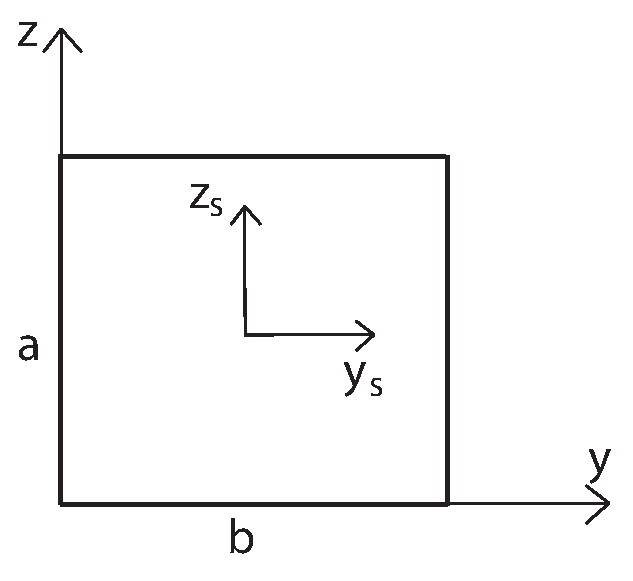
\includegraphics[width=2.5cm]{img/FTM_Viereck}
							\hspace{.75cm}
							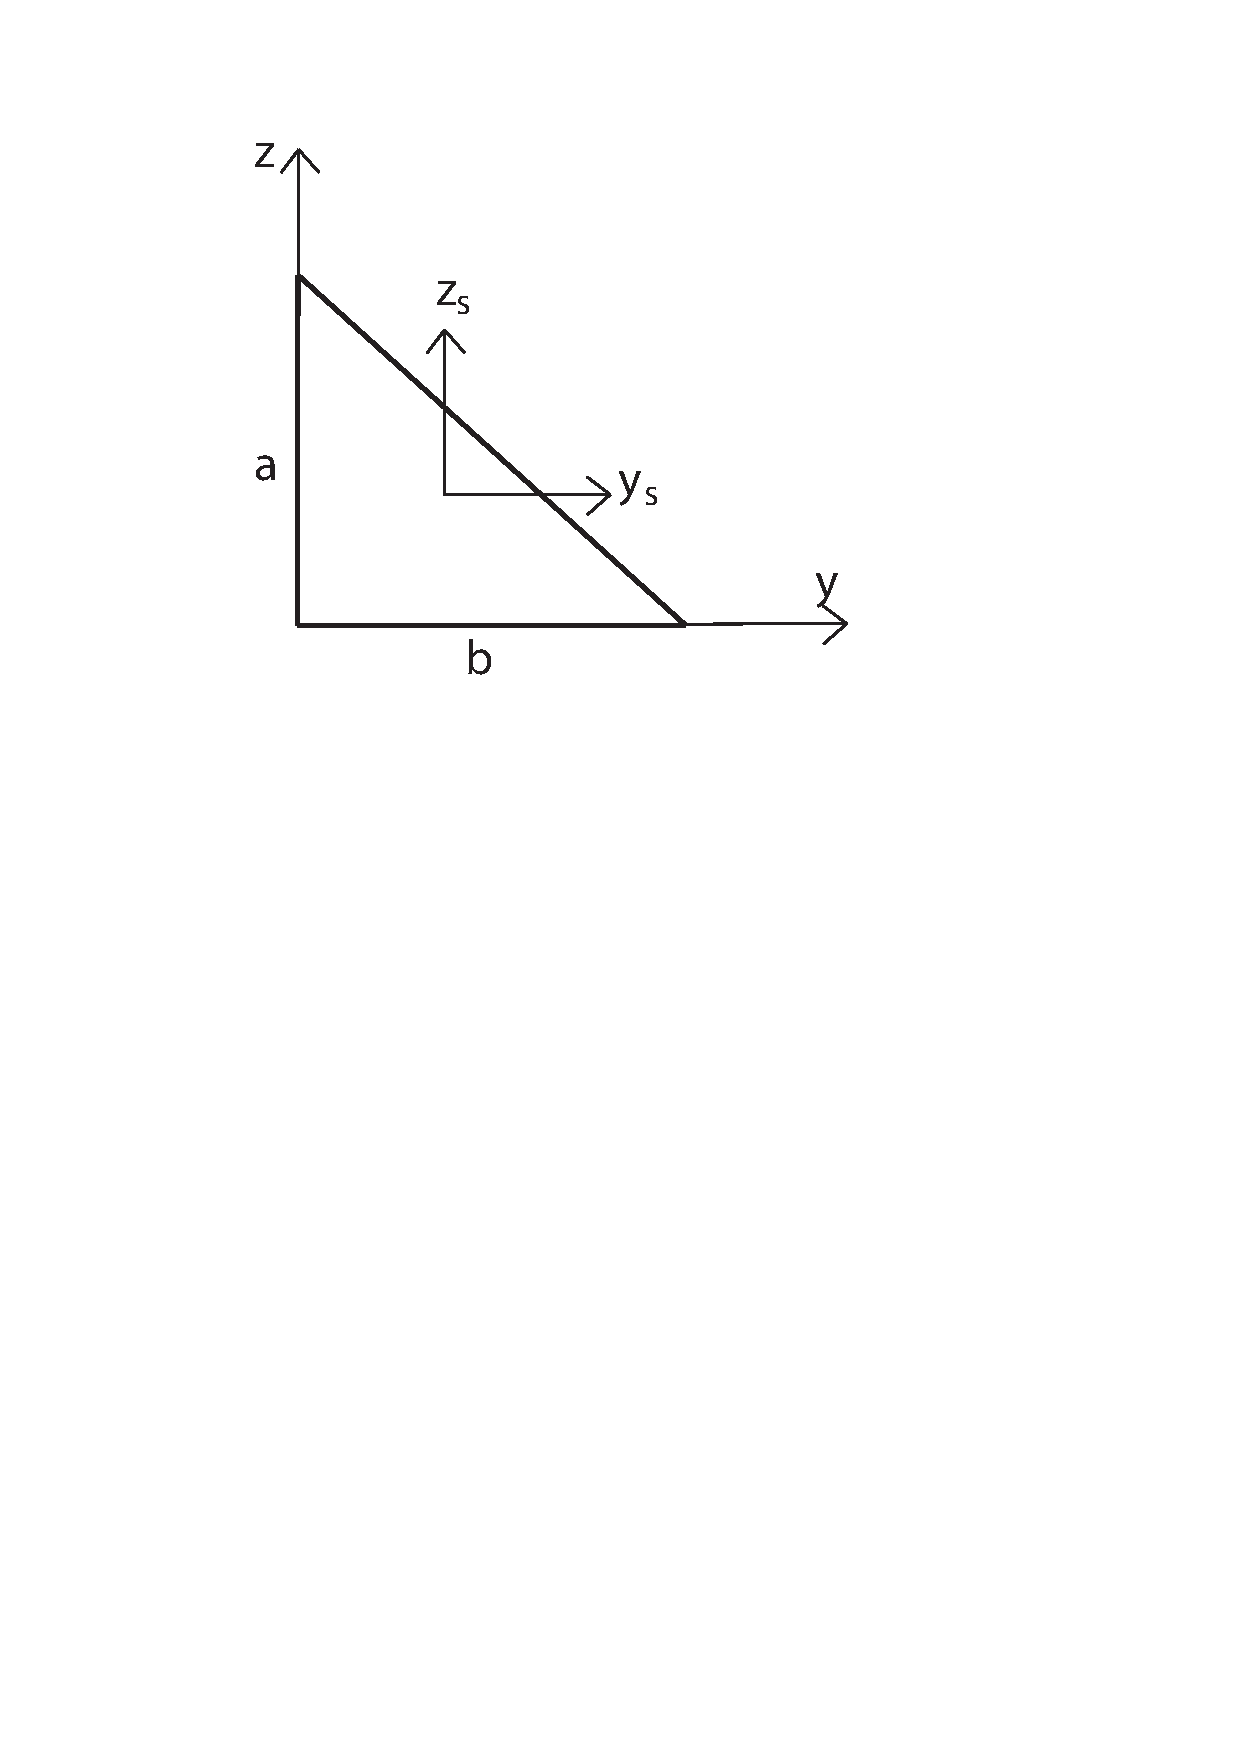
\includegraphics[width=2.5cm]{img/FTM_Dreieck}
						\end{center}
						
						\begin{description}
							\item[Viereck:]
								0 in S:
								\[
									\begin{array}{r@{\:=\:}l@{\ ,\ }r@{\:=\:}l@{\ ,\ }r@{\:=\:}l}
										I_{y_s} & \frac{a^3 b}{12} &
										I_{z_s} & \frac{a b^3}{12} &
										C_{y_s z_s} & 0
									\end{array}
								\]
								0 in Ecke:
								\[
									\begin{array}{r@{\:=\:}l@{\ ,\ }r@{\:=\:}l@{\ ,\ }r@{\:=\:}l}
										I_y & \frac{a^3 b}{3} & 
										I_z & \frac{a b^3}{3} & 
										C_{yz} & - \frac{a^2 b^2}{4}
									\end{array}
								\]
							\item[Kreis:] 
								\[
									I_P = \frac{\pi R^4}{2},\ 
									I_{y_s} = I_{z_s} = \frac{\pi R^4}{4},\ 
									C_{y_s z_s} = 0
								\]
							\item[Rohr:] $r$: innerer Radius 
								\begin{gather*}
									I_P = \frac{\pi (R^4 - r^4)}{2},\ 
									C_{y_s z_s} = 0 \\
									I_{y_s} = I_{z_s} = \frac{\pi (R^4 - r^4)}{4}
								\end{gather*}
							\item[Dreieck:]
									0 in S:
									\begin{gather*}
										I_{y_s} = \frac{a^3 b}{36} ,\ 
										I_{z_s} = \frac{a b^3}{36} \\
										C_{y_s z_s} = \frac{a^2 b^2}{72}
									\end{gather*}
									0 im rechten Winkel:
									\begin{gather*}
										I_y = \frac{a^3 b}{12} ,\ 
										I_z = \frac{a b^3}{12} \\ 
										C_{yz} = - \frac{a^2 b^2}{24}
									\end{gather*}
						\end{description}
					% Einige Flächenträgheitsmomente (end)
				% Flächenträgheitsmoment (end)
				\subsubsection{Wiederstandsmoment} % (fold)
					\begin{gather*}
						W_z = \frac{I_z}{||y||}
						\\
						W_P = \frac{I_P}{R}
					\end{gather*}
					Je grösser Wiederstandsmoment, desto kleiner die grösste Spannung.
				% Wiederstandsmoment (end)
				\subsubsection{Mohr'scher Kreis} % (fold)
					Symmetrieachse = Hauptachse
					\[
						Y=\mbox{\tiny $\left(\begin{array}{c}
							I_y \\
							\mathbf{+} C_{yz}
						\end{array}\right)$}
						,\
						Z=\mbox{\tiny $\left(\begin{array}{c}
							I_z \\
							\mathbf{-} C_{yz}
						\end{array}\right)$}
					\]
				% Mohrscher Kreis (end)
				\subsubsection{Spezielle Biegung} % (fold)
					\[
						N = T = 0
					\]
					\[
						M_b = \text{konst.,  auf Hauptachse des Querschnitts}
					\]
						
					\[
						\sigma_x = - \frac{M_b}{I_z} \cdot y
					\]
					
					\begin{wrapfigure}{l}{2.75cm}
						\begin{empheq}[box=\shadowbox*]{equation*}
						v(x)'' = \frac{M_b(x)}{EI_z}
					\end{empheq}
					\end{wrapfigure}
					
					\begin{wrapfigure}{r}{3cm}
						\vspace{-1.5cm}
						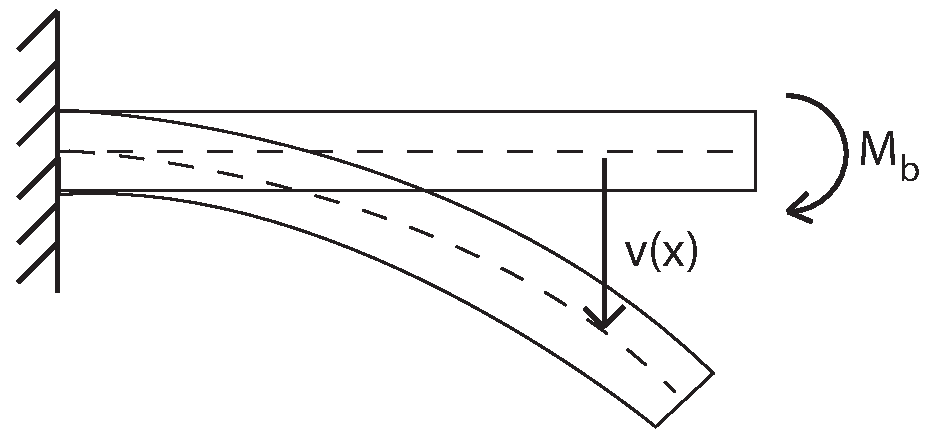
\includegraphics[width=3cm]{img/spezielle_Biegung_2}
						\vspace{-1.5cm}
					\end{wrapfigure}
					
					\[
						\beta = E I_z
					\]
					
					\[
						v' = \alpha \text{ (Winkel)}
					\]
					
				% Spezielle Biegung (end)
				\subsubsection{Spezielle Biegung und Zug oder Druck} % (fold)
					\begin{gather*}
						\sigma_x = \frac{N}{A} - \frac{M_b}{I_z} y
						\\
						u' = \frac{N}{AE}
						\\
						\varepsilon_x = -v'' y + u'
					\end{gather*}
					
					\begin{center}
						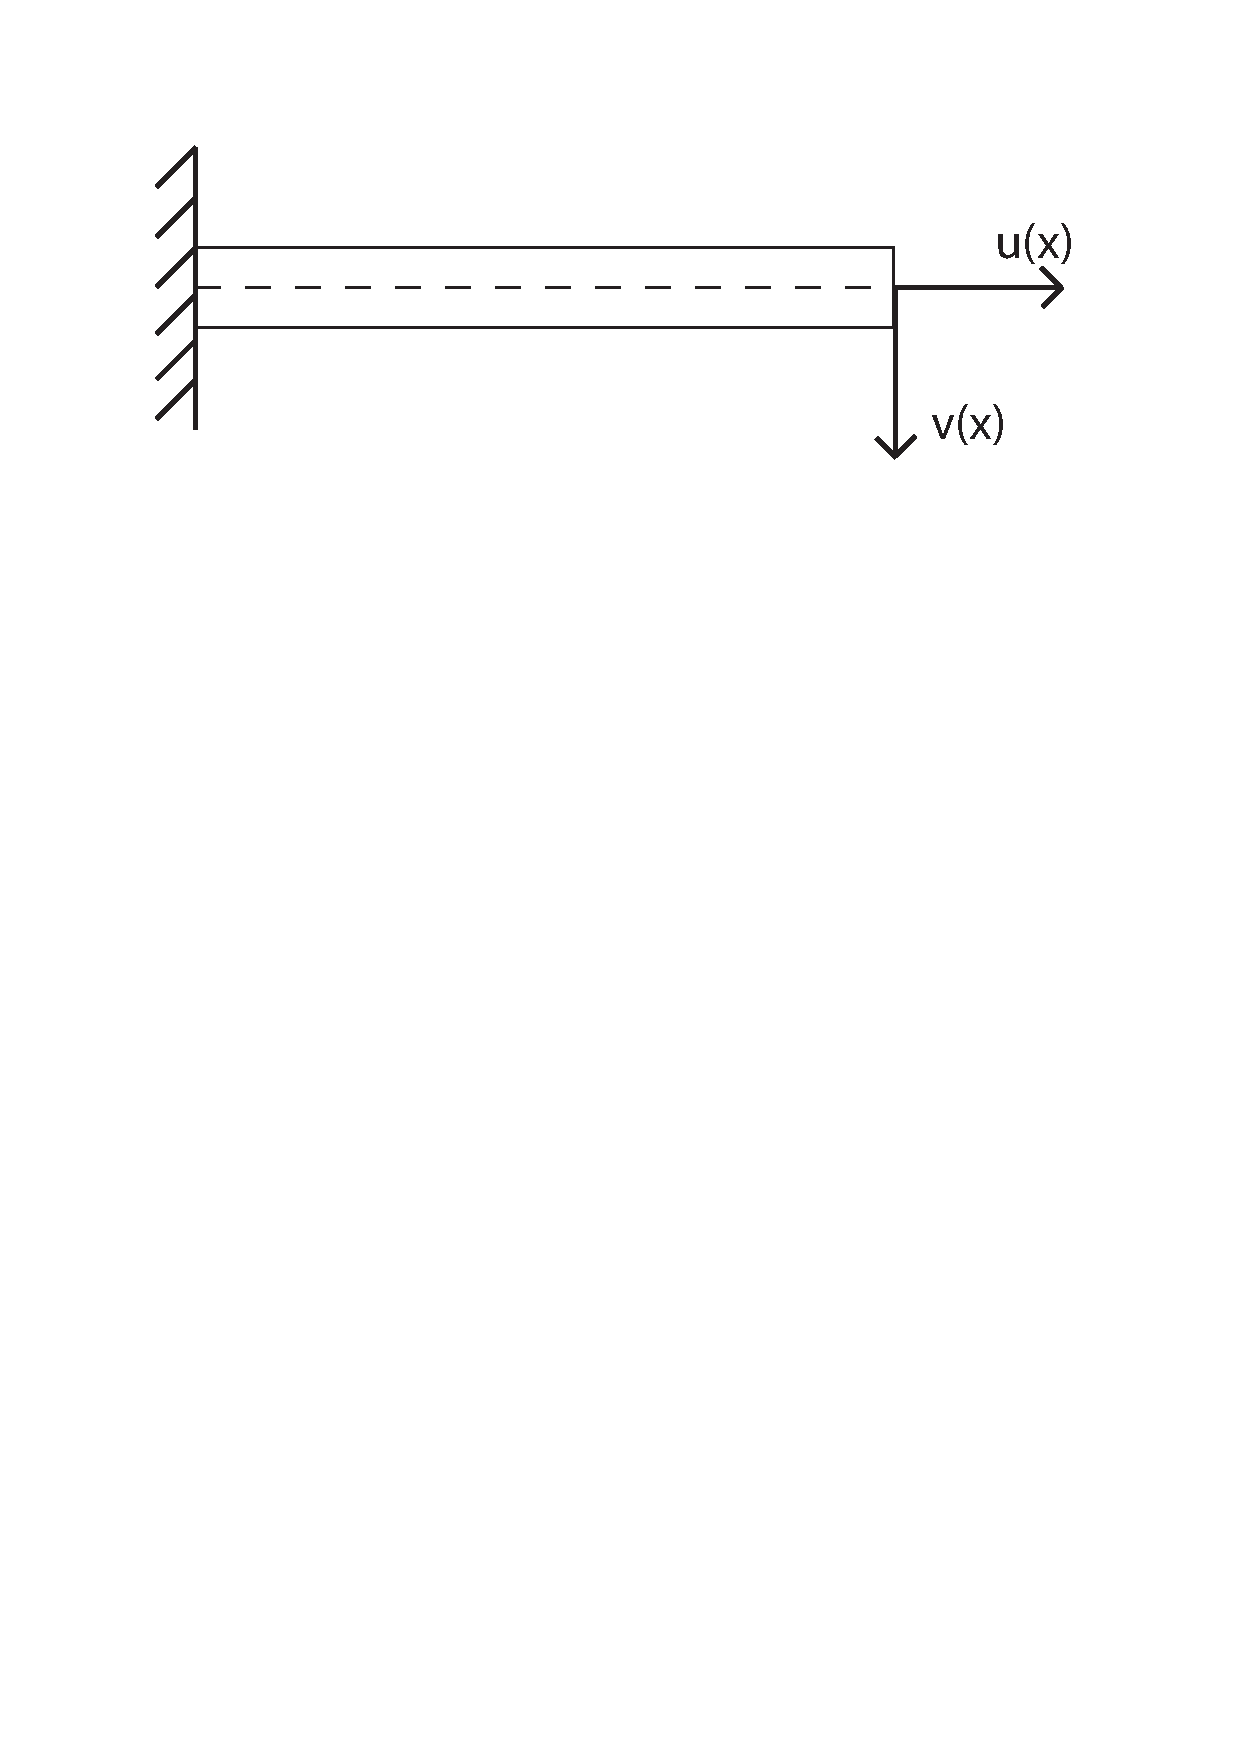
\includegraphics[width=3cm]{img/spezielle_Biegung_1}
					\end{center}
					
					Neutralachse mit $\sigma_x = 0$ um $y_n$ verschoben:
					\[
						y_n = \frac{N I_z}{M_b A}
					\]
				% Schiefe Biegung (end)
				\subsubsection{Schiefe Biegung} % (fold)
					Vektor des Biegemoments liegt nicht auf einer Hauptachse des Querschnitts. Hauptachsen anhand Mohr'scher Kreis berechnen.
					
					Biegemoment auf Hauptachsen aufgeteilt:
					\[
						\underline{M}_b = M_2 \underline{e}_2 + M_3 \underline{e}_3
					\]
					\[
						\sigma_x = \underbrace{- \frac{M_3}{I_3}x_2}_{\sigma_x^{M_3}} + \underbrace{\frac{M_2}{I_2}x_3}_{\sigma_x^{M_2}}
					\]
					Verschiebungen: \[
						u_2'' = \frac{M_3}{EI_3} \ ,\quad
						u_3'' = - \frac{M_2}{EI_2}
					\]
					Vektor der Durchbiegung: \[
						\underline{u} = u_2\underline{e}_2 + u_3\underline{e}_3
					\]
				% Schiefe Biegung (end)
				\subsubsection{Schubspannung infolge Biegung} % (fold)
					\paragraph{Flächenmoment 1. Grades:} % (fold)
						\begin{gather*}
							H_z = \iint \eta \ud A = y_{C'} \Delta A(y) \\
							\tau_{yx} = \tau_{xy} = \frac{Q}{I_z} \frac{H_z}{b}
						\end{gather*}
						\begin{center}
							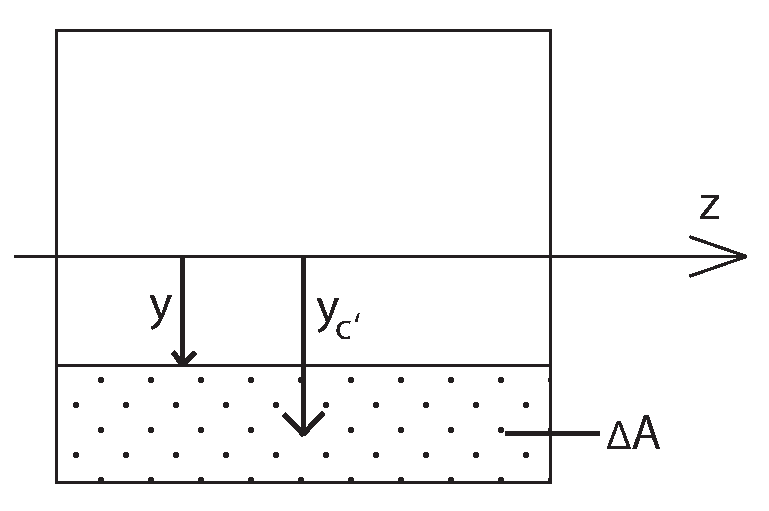
\includegraphics[width=3cm]{img/HZ}
						\end{center}
					% Flächenmoment 1. Grades (end)
				% Schubspannung infolge Biegung (end)
			% Biegeprobleme (end)
			\subsection{Torsion} % (fold)
				\begin{gather*}
					T = \iint \tau_{\phi x} r^2 \ud r \ud \phi
					\\
					\tau_{\varphi x}(r) = \frac{T}{I_P} r
				\end{gather*}
				
				Spezifischer Verdrehungswinkel:
				\[
					\vartheta ' = \frac{T}{GI_P}
				\]
			
				Verdrehungswinkel:
				\[
					\vartheta = \int_0^L \frac{T(x)}{GI_P} \ud x = \frac{TL}{GI_P}
				\]
			% Torsion (end)
			\subsection{Methode der finiten Elemente (FEM)} % (fold)
				\[
					[C] \{\Delta\} = \{P\}
				\]
				\begin{description}
					\item[$\lbrack C \rbrack:$] globale Steifigkeitsmatrix durch Überlagerung von
					\[
						[C^e] = \frac{EI}{\lambda^3} \left[\begin{array}{rrrr}
							12 & 6 & -12 & 6 \\
							6 & 4 & -6 & 2 \\
							-12 & -6 & 12 & -6 \\
							6 & 2 & -6 & 4
						\end{array}\right]
					\]
					\item[$\{\Delta\}:$] globaler Verschiebungsvektor
					\item[$\{P\}:$] globaler Kraftvektor
				\end{description}
				\[
					\{\Delta\} = \left(\begin{array}{c}
						v_1 \\
						\lambda \alpha_1 \\
						v_2 \\
						\lambda \alpha_2 \\
						\vdots \\
						v_n \\
						\lambda \alpha_n
					\end{array}\right) \ ,\quad
					\{P\} = \left(\begin{array}{c}
						P_1 \\
						M_1 / \lambda \\
						P_2 \\
						M_2 / \lambda \\
						\vdots \\
						P_n \\
						M_n / \lambda
					\end{array}\right)
				\]
				
				\begin{center}
					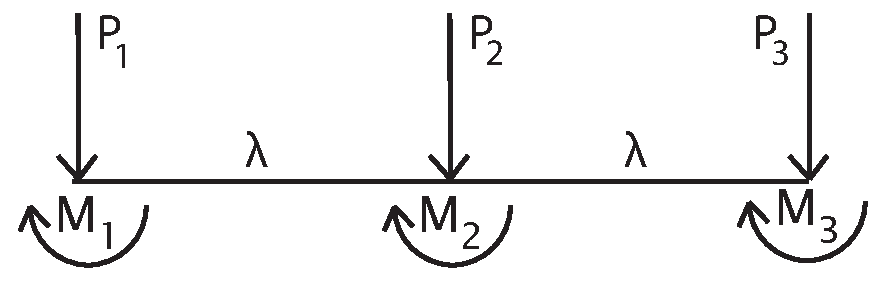
\includegraphics[width=4cm]{img/FEM}
				\end{center}
			% Methode der finiten Elemente (FEM) (end)
			\subsection{Arbeit und Deformationsenergie} % (fold)
				\[
					\mathcal{W} =
					\int_{t_1}^{t_2} \mathcal{P} \ud t = 
					\int_{t_1}^{t_2} \underline{F} \cdot \underline{v} \ud t = 
					\int_P^Q \underline{F} \cdot \ud \underline{r}
				\]
				\subsubsection{Deformationsenergie} % (fold)
					\[
						U_{\mbox{\tiny Feder}} = V(x) = \frac{1}{2} k x^2
					\]
					$V$ im entlasteten Zustand ($V(x_0) = 0$), $k$ ist Federkonstante.

					\begin{align*}
						U_{\mbox{\tiny Zug/Druck}} &= \int_0^L \frac{N^2 (x)}{2AE} \ud x \\
						&= \frac{1}{2} \int_0^L AE \cdot \varepsilon_x^2 (x) \ud x
					\end{align*}
					
					\begin{align*}
						U_{\mbox{\tiny Biegung}} &= \int_0^L \frac{M_b^2 (x)}{2EI_z} \ud x \\
						&= \frac{1}{2} \int_0^L EI_z \cdot v''(x)^2 \ud x
					\end{align*}
					
					Bei \emph{schiefer Biegung}:
					\[
						U_{\mbox{\tiny Biegung}} = \int_0^L \left[ \frac{M_2^2 (x)}{2EI_2} + \frac{M_3^2 (x)}{2EI_3} \right] \ud x
					\]
					
					\begin{align*}
						U_{\mbox{\tiny Torsion}} &= \int_0^L \frac{T^2(x)}{2GI_P} \ud x \\
						&= \frac{1}{2} \int_0^L GI_P \cdot \vartheta'(x)^2 \ud x
					\end{align*}
					
					\paragraph{Zusammengesetzte Beanspruchung:} % (fold)
						Summe aller einzelnen auftretenden Energien:
						\[
							U_{\mbox{\tiny Total}}
							= U_{\mbox{\tiny Feder}}
							+ U_{\mbox{\tiny Zug/Druck}}
							+ U_{\mbox{\tiny Biegung}}
							+ U_{\mbox{\tiny Torsion}}
						\]
					% Zusammengesetzte Beanspruchung (end)
				% Deformationsenergie (end)
				\subsubsection{Die Arbeitsgleichung} % (fold)
					\paragraph{Statisch bestimmtes Problem:} % (fold)
						Gesucht: Verschiebung $v(a)$ oder $\alpha(b)$
						\begin{enumerate}
							\item sbEp bestimmen, Einheitskraft bei $x=a$
							bzw. Einheitsmoments bei $x=b$ einführen
							\item $\overline{M}_b(x)$ am sbEp bestimmen
							\item $M_b(x)$ am gegebenen Problem bestimmen
							\item \[
								\left.
								\begin{array}{r}
								v(a) \\
								\alpha(b)
								\end{array}
								\right\}
								 = \int_0^L \overline{M}_b(x) \frac{M_b(x)}{EI_z} \ud x
							\]
							Bei \textbf{zusammengesetzter Beanspruchung} rechte Seite ergänzen mit:
							\[
								\int_0^L \overline{N}(x) \frac{N(x)}{EA} \ud x + \int_0^L \overline{T}(x) \frac{T(x)}{GI_P} \ud x
							\]
						\end{enumerate}
					% Statisch bestimmte Probleme (end)
					\paragraph{Statisch unbestimmtes Problem:} % (fold)
						\begin{enumerate}
							\item $n$-fach statisch unbestimmt
							\item $n$ Bindungen lösen
							\item $n$ sbEp einführen
							\item Für jedes sbEp bekommt man eine zusätzliche Gleichung zur Bestimmung der Lagerkräfte:
							\[
								\int_0^L \overline{M}_b(x) \frac{M_b(x)}{EI_z} \ud x = 0
							\]
						\end{enumerate}
					% Statisch unbestimmtes Problem (end)
				% Die Arbeitsgleichung (end)
				\subsubsection{Satz von Castigliano} % (fold)
					\paragraph{Statisch bestimmtes Problem:} % (fold)
						\textbf{Verschiebung} $v_k$ in Kraftrichtung wo $F_k$ angreift:
						\[
							v_k = \frac{\partial U}{\partial F_k}
						\]
						
						Beispiel:
						\begin{align*}
							v_k &= \frac{\partial}{\partial F_k} \int_0^L \frac{M_b^2(x)}{2EI_z} \ud x \\
							&= \int_0^L \frac{M_b(x)}{EI_z} \frac{\partial M_b(x)}{\partial F_k} \ud x
						\end{align*}
						
						\textbf{Verdrehung} $\alpha_i$ in Richtung eines Einzelmoments $M_i$:
						\[
							\alpha_i = \frac{\partial U}{\partial M_i}
						\]
						
						Beispiel:
						\begin{align*}
							\alpha_i &= \frac{\partial}{\partial T_i} \int_0^L \frac{T^2(x)}{2GI_P} \ud x \\
							&= \int_0^L \frac{T(x)}{GI_P} \frac{\partial T(x)}{\partial T_i} \ud x
						\end{align*}
						
						\textbf{Verschiebung} $v_H$ bzw. $\alpha_H$ an \textbf{lastfreien Stelle}:
						\begin{enumerate}
							\item Hilfskraft $H$ bzw. Hilfsmoment $M_H$ an der lastfreien Stelle einführen
							\item Berechnung der Deformationsenergie inkl. Hilfsgrösse
							\item Kraft nach der partiell abgeleitet wird muss eindeutig
							bezeichnet sein. Gibt es zwei Kräfte mit Betrag $F$, müssen sie
							zu $F_1$ und $F_2$ umbenannt werden.
							\begin{align*}
								v_H &= \left(\frac{\partial U}{\partial H}\right)_{H=0} \\
								\alpha_i &= \left(\frac{\partial U}{\partial M_H}\right)_{M_H=0}
							\end{align*}
						\end{enumerate}
					% Statisch bestimmte Probleme (end)
					\paragraph{Statisch unbestimmtes Problem:} % (fold)
						\begin{enumerate}
							\item $n$-fach statisch unbestimmt
							\item $n$ Bindungen lösen
							\item Bindungskräfte als äussere Lasten einführen
							\item $n$ zusätzliche Gleichungen zur Bestimmung der Lagerkräfte:
							\begin{align*}
								v_H &= \left(\frac{\partial U}{\partial F_k}\right) = 0 \\
								\alpha_i &= \left(\frac{\partial U}{\partial M_H}\right) = 0
							\end{align*}
						\end{enumerate}
					% Statisch unbestimmtes Problem (end)
				% Satz von Castigliano (end)
			% Arbeit und Deformationsenergie (end)
			\subsection{Knickung} % (fold)
				\emph{Bei zusammengesetzter Beanspruchung:}
				Stabilitätsproblem wenn $|M_{b_{\text{undef}}}| < |M_{b_{\text{def}}}$
				
				\paragraph{Stabilitätsgrenze/“Eulersche Knicklast”:} % (fold)
					\[
						F_E = k \cdot \frac{\pi^2 EI_z}{L^2}
					\]
				
					\begin{center}
						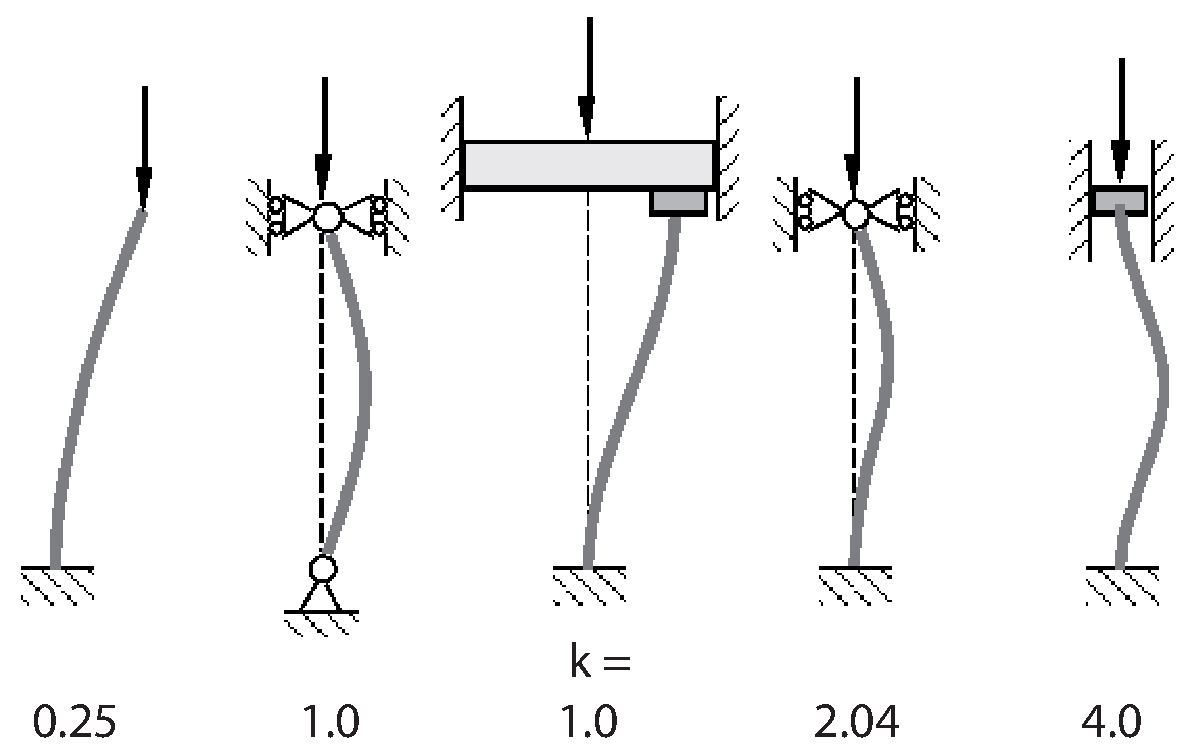
\includegraphics[width=4.5cm]{img/Knickung}
					\end{center}
				
					Für alle Stäbe unter Drucklast muss das System auf Stabilität überprüft werden:
					\begin{gather*}
						\text{falls Stabkraft } S < F_E \\
						\Rightarrow \text{System stabil}
					\end{gather*}
				% Stabilitätsgrenze/Eulersche Knicklast (end)
			% Knickung (end)
		% Deformierbare Körper (end)
	\end{multicols*}
\end{document}






























